\documentclass[11pt,a4paper]{article}
\usepackage[T1]{fontenc}
\usepackage[utf8]{inputenc}
\usepackage{lmodern}
\usepackage{amsmath,amssymb,amsthm,mathtools,mathrsfs}
\usepackage{graphicx,float,xcolor,multicol}
\usepackage[shortlabels]{enumitem}
\usepackage[margin=27mm]{geometry}
\usepackage{microtype,needspace,placeins}
\usepackage{tikz,tikz-cd}
\usetikzlibrary{arrows.meta,calc,positioning,patterns,decorations.pathreplacing}
\usepackage[colorlinks=true,linkcolor=teal,urlcolor=teal,citecolor=teal]{hyperref}
\setlength{\parindent}{0pt}
\setlength{\parskip}{.6em}
\setcounter{secnumdepth}{0}
\allowdisplaybreaks
\raggedbottom
\providecommand{\cross}{\times}
\DeclareUnicodeCharacter{2020}{\ensuremath{\dagger}}
\DeclareMathOperator{\supp}{supp}
\DeclareMathOperator*{\esssup}{ess\,sup}
\providecommand{\chapter}{\section}
\newenvironment{tool}[2]{\subsection*{Tool #1 --- #2}}{}
\newcommand{\ToolRef}[1]{Tool #1}
\newcommand{\FigureTag}[2]{\textit{Figure #1}}
\newcommand{\Result}[1]{\subsection*{#1}}
\newcommand{\Application}[1]{\subsubsection*{Application\if\relax\detokenize{#1}\relax\else\space--- #1\fi}}
\newcommand{\ProofHeading}{\par\textit{Proof.}\space}
\newcommand{\ProofOf}[1]{\par\textit{Proof of #1.}\space}
\newcommand{\RemarkHeading}{\par\textbf{Remark.}\space}
\newcommand{\NoteHeading}{\par\textbf{Note.}\space}
\newcommand{\ExerciseHeading}{\par\textbf{Exercise.}\space}

\graphicspath{{figures/mcmullens-surgery/}}
\begin{document}
\section*{McMullen's Surgery III: Commuting Deformations and Finite Symmetry}
% BLOG-CONTENT-BEGIN
\begin{center}
\emph{McMullen's Surgery:}
\BlogPost{third-surgery}{Part I} \(\,\cdot\,\)
\BlogPost{mcmullens-surgery}{Part II} \(\,\cdot\,\) Part III
\end{center}

In \BlogPost{mcmullens-surgery}{Part II}, we obtained the rational map $g$ and a stable conjugacy $(C,f)\sim(J(g),g)$. We retain $C$, $f$, and $g$ here.

\subsection*{Proposition 6.25}: Suppose $C$ carries no invariant line field. Then $\text{Mod}(J(g), g) \cong \text{Aut}(g)$, and consequently $\text{Mod}(C, f)$ is a finite group.


   \textit{Proof.}: The stable conjugacy transports invariant line fields between $C$ and $J(g)$, so $J(g)$ carries no invariant line field. Let $\phi$ be an element of $\text{Mod}(J(g), g)$. We claim the ideal boundary values of $\phi$ on any component of $I(J(g))$ coincide with those of a conformal map commuting with $g$. If so, by \BlogPost{third-surgery}{Proposition $6.8$ and Corollary $6.9$} there is an isotopy connecting $\phi$ to a unique quasiconformal map $\hat{\phi}$ which is conformal on $\hat{\mathbb{C}}\backslash J(g)$ and commutes with $g$ everywhere. The Beltrami coefficient of $\hat{\phi}$ is $g$-invariant and supported on $J(g)$. Since $J(g)$ carries no invariant line field, this coefficient must vanish almost everywhere. Hence $[\phi]$ is represented by an element of $\text{Aut}(g)$, completing the proof.\\ To establish the claim, replace $g$ by a suitable iterate so that every periodic complementary component is fixed. If there are no such components, the claim is vacuous. By our classification theorem, each fixed component is a Siegel disk, a parabolic basin, or a superattracting basin, and is conjugate to a rigid model after uniformization. \\
   On the ideal boundary of each fixed component $U$, $\phi$ therefore conjugates the rigid model on $U$ to the rigid model on $\phi(U)$. As remarked earlier, the two models must be identical, and up to composition with uniformizing maps, $\phi$ is a rotation commuting with the dynamics throughout the disk. Thus the ideal boundary values of $\phi$ coincide with those of a conformal map commuting with $g$.\\
   Now let $U$ be a preperiodic component, and let $V = \phi(U)$. There is a least integer $k$ such that $g^{\circ k}(U)$ and $g^{\circ k}(V)$ are components fixed by $g$. If $g^{\circ k}$ maps $U$ by degree $1$, as $g^{\circ k}(U)$ and $g^{\circ k}(V)$ are fixed, one can replace $\phi$ there with a conformal map $\tilde{\phi}:g^{\circ k}(U)\rightarrow g^{\circ k}(V)$ without changing the ideal boundary values. The conformal replacement on $U$ is $(g^{\circ k}\big|_V)^{-1}\circ\tilde{\phi}\circ(g^{\circ k}\big|_U)$.\\
   On the other hand, if $\text{deg}(g^{\circ k}\big|_U)>1$, then by construction the restrictions of $g^{\circ k}$ to $U$ and $V$ have a unique critical value, which either coincides with the center of a Siegel disk or with the distinguished critical point in a parabolic or superattracting basin. The conformal map $\tilde{\phi}$ carries one critical value to the other and can therefore be lifted through the two proper maps. Thus suitable conformal replacements can be arranged in this case as well.


   Before talking about Conjecture $6.4$, let us briefly talk about buried sets. Indeed, an invariant Julia component need not meet the boundary of any Fatou component.

   \subsection*{Definition 6.26}{(Buried Sets)}: A subset of a closed set $J \subset X$ will be called buried if none of its points belongs to the boundary of a component of $X\backslash J$.


   Classical examples of buried sets arise from Cantor-like sets. A Cantor set in an interval has only countably many complementary intervals and hence only countably many boundary endpoints; the Cantor set being uncountable, it must have uncountably many buried points. A standard example of buried Julia components is given in the following proposition (proved in \cite{mcmullen1988automorphisms}); more information on buried Julia components can be found in \cite{godillon2015family} and \cite{wang2022buried}.

   \subsection*{Proposition 6.27}: Let $f(z) = z^2 + \frac{\lambda}{z^3}$. For all non-zero $\lambda$ sufficiently small,
   \begin{enumerate}
       \item $J(f)$ has uncountably many buried components.
       \item $J(f)$ has a unique forward invariant buried component.
       \item $J(f)$ is homeomorphic to (a Cantor set) $\times$ $\mathbb{S}^1$
   \end{enumerate}

    \begin{figure}[H]\centering
    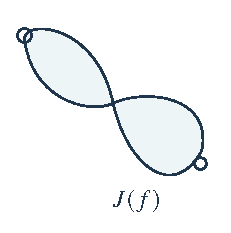
\includegraphics[width=5.5cm]{ms-fig-31.pdf}
    \FigureTag{MS31}{fig:ms-31}
    \end{figure}


   \subsection*{Definition 6.28}{(Exposed Critical Points)}: We say $f(z)$ has exposed critical points if every critical point lies in the Fatou set $F(f)$ or on the boundary of a component of $F(f)$.


   In proving the special case of Conjecture $6.4$ the following special case of a result of Strebel found in \cite{MR505549} was used. We shall state the special case here.

   \subsection*{Theorem 6.29}{(Strebel's Theorem)}: Let $U$ be a finitely connected domain in $\hat{\mathbb{C}}$, and let $\phi:\overline{U} \rightarrow \overline{U}$ be a quasiconformal homeomorphism which is identity on $\partial U$. Then there is a unique quasiconformal map $\psi$ of minimal dilatation among those isotopic to $\phi$ (relative to $\partial U$). The absolute value of the Beltrami differential $|\psi_{\bar{z}}/\psi_z|$ is constant on $U$ (in fact, $\psi$ is a Teichm\"uller mapping of finite norm).



   Now we shall state a final theorem related to the difficult question of the existence of invariant line fields (explained in \cite{mcmullen1994frontiers} and \cite{mcmullen2016complex}). The uniqueness in Strebel's Theorem is the ingredient that controls stable conjugacies when the critical points are exposed.

   \subsection*{Theorem 6.30}: If $J(f)$ is connected and $f$ has exposed critical points, then $\text{Mod}(J(f), f)$ is a finite group \cite{mcmullen1988automorphisms}.

   Thus, for rational maps with exposed critical points, the finiteness predicted by Conjecture $6.4$ follows.

% BLOG-CONTENT-END
\bibliographystyle{amsalpha}
\bibliography{tools/profiles/surgeries/MSc_Dissertation}
\end{document}
